% SASYR 2025 - Template based on:
% samplepaper.tex, a sample chapter demonstrating the
% LLNCS macro package for Springer Computer Science proceedings;
% Version 2.20 of 2017/10/04
%
\documentclass[runningheads]{llncs}
%
\usepackage{graphicx}
\usepackage{lipsum}
\usepackage{url}
% Used for displaying a sample figure. If possible, figure files should
% be included in EPS format.
%
% If you use the hyperref package, please uncomment the following line
% to display URLs in blue roman font according to Springer's eBook style:
% \renewcommand\UrlFont{\color{blue}\rmfamily}

\begin{document}
%
\title{NCAA March Madness 2026 Forecasting: A Two-Stage Machine Learning System for Tournament Selection and Bracket Outcomes (Men's + Women's)}
%
%\titlerunning{Abbreviated paper title}
%\section{% If the paper title is too long for the running head, you can set}
% an abbreviated paper title here
%
\author{
Clark Everson \email{(cmeverson@uchicago.edu)}\and
Brooke Rios \email{(brios@uchicago.edu)} \and
Sovin Birla \email{(sovin@uchicago.edu)} \and
Hoang Bui \email{(hoangbui@uchicago.edu)} \and
Amber Keahy \email{(akeahey@uchicago.edu)}
}
%
%
\maketitle              % typeset the header of the contribution
%
\begin{abstract}
Accurate forecasting of the NCAA March Madness tournament presents a dual-regime machine learning challenge. We propose a production-ready, two-stage system: \textbf{Task A: Selection Prediction} (team-season classification to determine the 68-team field) and \textbf{Task B: Bracket Outcome Prediction} (game-level probabilistic classification conditional on the field). The system is run separately for Men’s (MBB) and Women’s (WBB) basketball, with an empirical test of structural sharing. We employ a rigorous data governance strategy, strictly holding out the 2026 season for final out-of-sample evaluation and deploying layered defenses against data leakage, a known risk in sports forecasting. Evaluation across a broad family of models, including Decision Trees, MLPs, and kernel-based methods, led to the selection of a pooled Decision Tree model for Selection (AUC 0.9963) and separate models for Bracket outcomes: an MLP for MBB (AUC 0.8497) and an autoencoder-proxy MLP for WBB (AUC 0.8878). Our results confirm that Selection behaves as a high-signal threshold classification problem, while Bracket prediction is an inherently probabilistic problem, with WBB exhibiting a stronger hierarchy signal than MBB. The resulting pipeline produces a coherent set of 2026 forecast artifacts for both leagues.\\
\end{abstract}

\section{Introduction}

The NCAA Division I Basketball Tournaments (March Madness) are a major global event, with predictive modeling playing a significant role in media, analytics, and sports betting. Existing approaches often treat tournament prediction as a single, monolithic problem. However, the system is fundamentally two distinct tasks with different units of analysis and underlying statistical regimes: selecting the field of teams, and predicting game-by-game outcomes.

This paper presents an end-to-end Machine Learning pipeline designed to address this duality. Our primary contributions are: \\
\textbf{1. Two-Stage Architecture}: Explicitly defining and modeling the selection (team-season classification) and bracket (game-level probabilistic classification) problems separately, demonstrating that this is the correct technical decomposition. \\
\textbf{2. Rigorous Temporal Validation and Leakage Defense}: Implementing rolling multi-season cross-validation and a strict 2026 holdout to ensure model generalization and protect against common pitfalls like data leakage. \\
\textbf{3. Empirical Comparison of Leagues}: Providing a side-by-side analysis of Men’s (MBB) and Women’s (WBB) leagues, confirming that the high-level discriminative structure for selection is shared (justifying pooling), but the probabilistic structure for bracket outcomes is different (justifying separate models). \\


\section{System Architecture and Problem Decomposition}
\subsection{Task A: Selection Prediction (Team Season Classification)}
This task aims to classify a team's season profile as either "Selected" or "Not Selected" into the tournament.

\subsection{Task B: Bracket Outcome Prediction (Game-Level Probabilistic Classification)} 

\section{Experimental Design and Data Governance}
\subsection{Data Sources and Feature Provenance}
\subsection{Validation Strategy and Leakage Defense}
\subsection{Evaluation Metrics} 

\section{Model Families and Final Selections}
We evaluated a diverse set of model families, including Logistic Regression, Linear/Kernel SVM, Decision Trees, Random Forests, Gradient Boosting (XGBoost-style), and basic Neural Networks (MLP), to cover a broad spectrum of inductive biases.
\begin{table}
    \centering
    \begin{tabular}{cccc}
        \textbf{Task} & \textbf{League(s)} & \textbf{Model} & \textbf{Key Metrics (2026 Holdout)} \\
        Selection & Pooled (MBB + WBB) & Decision Tree & 
        \begin{itemize}
            \item AUC 0.996324 \\
            \item PR-AUC 0.994024 \\
            \item Precision@K 0.992647 \\
        \end{itemize}
        Bracket & MBB & Multi-Layer Perceptron (MLP) & AUC 0.849678 \\
        Bracket & WBB & Autoencoder-Proxy MLP & AUC 0.887775 \\
    \end{tabular}
    \caption{Final Locked Model Architecture}
    \label{tab:placeholder}
\end{table}

The pooled selection model was chosen because empirical testing showed negligible performance delta between pooled and separate league models, suggesting the selection boundary structure is shared. Separate bracket models were justified by observed structural differences in EDA and validation
\section{Results and Analysis}
\subsection{Differences between MBB and WBB}
Our comparative analysis confirms that WBB exhibits a stronger hierarchy signal.
\begin{itemize}
    \item \textbf{WBB Predictability:} WBB bracket outcomes were more predictable (higher AUC 0.8878 vs. 0.8497 for MBB). The win probability curves conditional on Elo differences were steeper, indicating that strength differentials translate more directly into win probability.
    \item \textbf{Model Selection:} This structural difference justified the use of a more flexible autoencoder-proxy MLP for WBB, which leverages representation learning, while a standard MLP was sufficient for MBB.
\end{itemize}
\subsection{Error Regimes}
Error analysis confirmed the expected pattern for strength-driven models:
\begin{itemize}
    \item \textbf{Selection Errors:} Concentrate overwhelmingly at the \textbf{bubble region} (teams near the selection cutoff), where committee heuristics and non-quantitative factors may be decisive.
    \item \textbf{Bracket Errors:} Concentrate at \textbf{small Elo gap games} ($ELO_{diff} \approx{0}$), confirming that these are the most uncertain matchups. Missed upset rates were significantly lower when Elo gaps exceeded 100, which aligns with the model's reliance on team strength.
\end{itemize}
\subsection{Calibration}
Calibration was critical for the probabilistic bracket task. Metrics (Log-Loss, Brier Score, ECE) confirmed that raw probabilities required calibration (e.g., Isotonic Regression) to ensure that predicted probabilities accurately reflect observed win frequencies, preventing distortion in tournament simulation.

\section{Conclusion and Final Work}

We successfully implemented a robust, two-stage machine learning system for NCAA March Madness forecasting. The architecture correctly decomposes the problem, and our validation strategy provides a defensible basis for the high evaluation metrics. The final pipeline delivers a repeatable, audited forecast, producing 2026 tournament field predictions, matchup probabilities, and simulation-based championship odds (projected champions: Miami (Ohio) for MBB, Connecticut for WBB). \\
Future work should focus on enriching the feature space in the bracket task, potentially by incorporating more complex interaction terms or dynamic features that capture form/momentum changes late in the season, to address the remaining variance in close-gap matchups.



\paragraph{Sample Heading (Fourth Level)}
The contribution should contain no more than four levels of
headings. Table~\ref{tab1} gives a summary of all heading levels.

\begin{table}
\caption{Table captions should be placed above the
tables.}\label{tab1}
\begin{tabular}{|l|l|l|}
\hline
Heading level &  Example & Font size and style\\
\hline
Title (centered) &  {\Large\bfseries Lecture Notes} & 14 point, bold\\
1st-level heading &  {\large\bfseries 1 Introduction} & 12 point, bold\\
2nd-level heading & {\bfseries 2.1 Printing Area} & 10 point, bold\\
3rd-level heading & {\bfseries Run-in Heading in Bold.} Text follows & 10 point, bold\\
4th-level heading & {\itshape Lowest Level Heading.} Text follows & 10 point, italic\\
\hline
\end{tabular}
\end{table}


\noindent Displayed equations are centered and set on a separate
line.
\begin{equation}
x + y = z
\end{equation}
Please try to avoid rasterized images for line-art diagrams and
schemas. Whenever possible, use vector graphics instead (see
Fig.~\ref{fig1}).

\begin{figure}
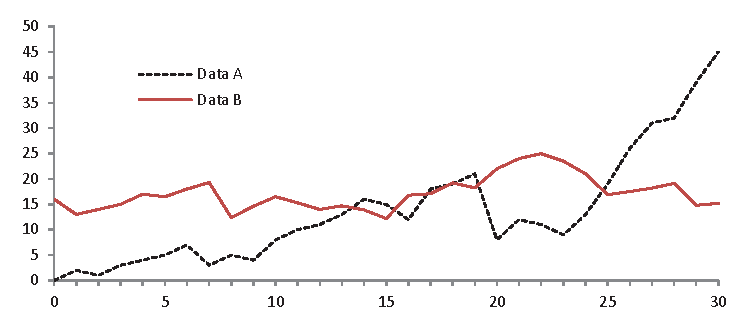
\includegraphics[width=\textwidth]{fig1.eps}
\caption{A figure caption is always placed below the illustration.
Please note that short captions are centered, while long ones are
justified by the macro package automatically.} \label{fig1}
\end{figure}

%
% the environments 'definition', 'lemma', 'proposition', 'corollary',
% 'remark', and 'example' are defined in the LLNCS documentclass as well.
%

For citations of references, use:
In \cite{einstein} Einstein....

In \cite{knuthwebsite} the authors

This \cite{latexcompanion} is Latex. 
%
% ---- Bibliography ----
%
% BibTeX users should specify bibliography style 'splncs04'.
% References will then be sorted and formatted in the correct style.
%
\bibliographystyle{refs-style}
\bibliography{refs}
%
\end{document}
